\section{COMPONENTE HARDWARE}

El componente hardware se ha implementado utilizando dos lenguajes de programación; \emph{Wiring} para el microprocesador ATmega32u4, Python para el procesador \emph{Atheros AR9331}.

\begin{figure}[H]
    \centering
    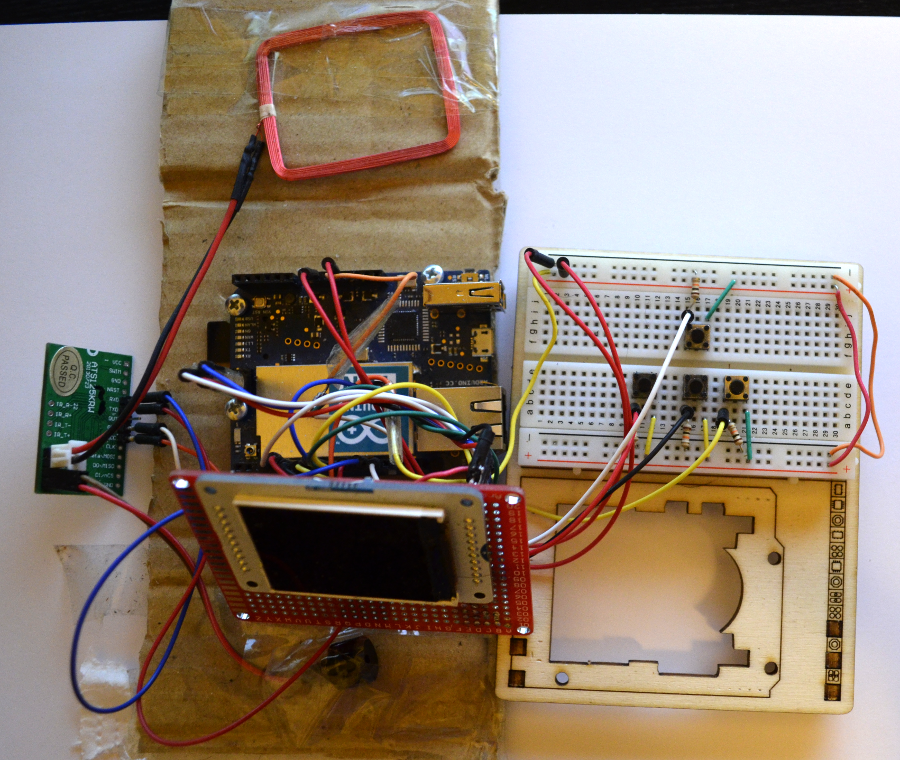
\includegraphics[keepaspectratio,width=0.8\textwidth]{lector_arduino.png}
    \caption{Lector Arduino}\label{fig:lector-arduino}
\end{figure}

\subsection{Configurando el sistema}

El primer paso es configurar la placa de Arduino Yún para empezar a trabajar sobre ella. Para ello Yún corre una distribución de Linux llamada \emph{OpenWrt-Yun}, basado en \emph{OpenWrt}, la cual nos permite acceder vía \emph{ssh} o vía web para poder configurarla.

La primera vez que se conecta Arduino Yún se crea una red sin encriptar para poder conectarnos a ella y poder configurarla, el nombre de la red tiene el formato \emph{ArduinoYun-XXXXXXXXXXXX}. Una vez conectados se accede al panel web de configuración a través de la url \emph{http://arduino.local} y se nos muestra la siguiente ventana:

\begin{figure}[H]
    \centering
    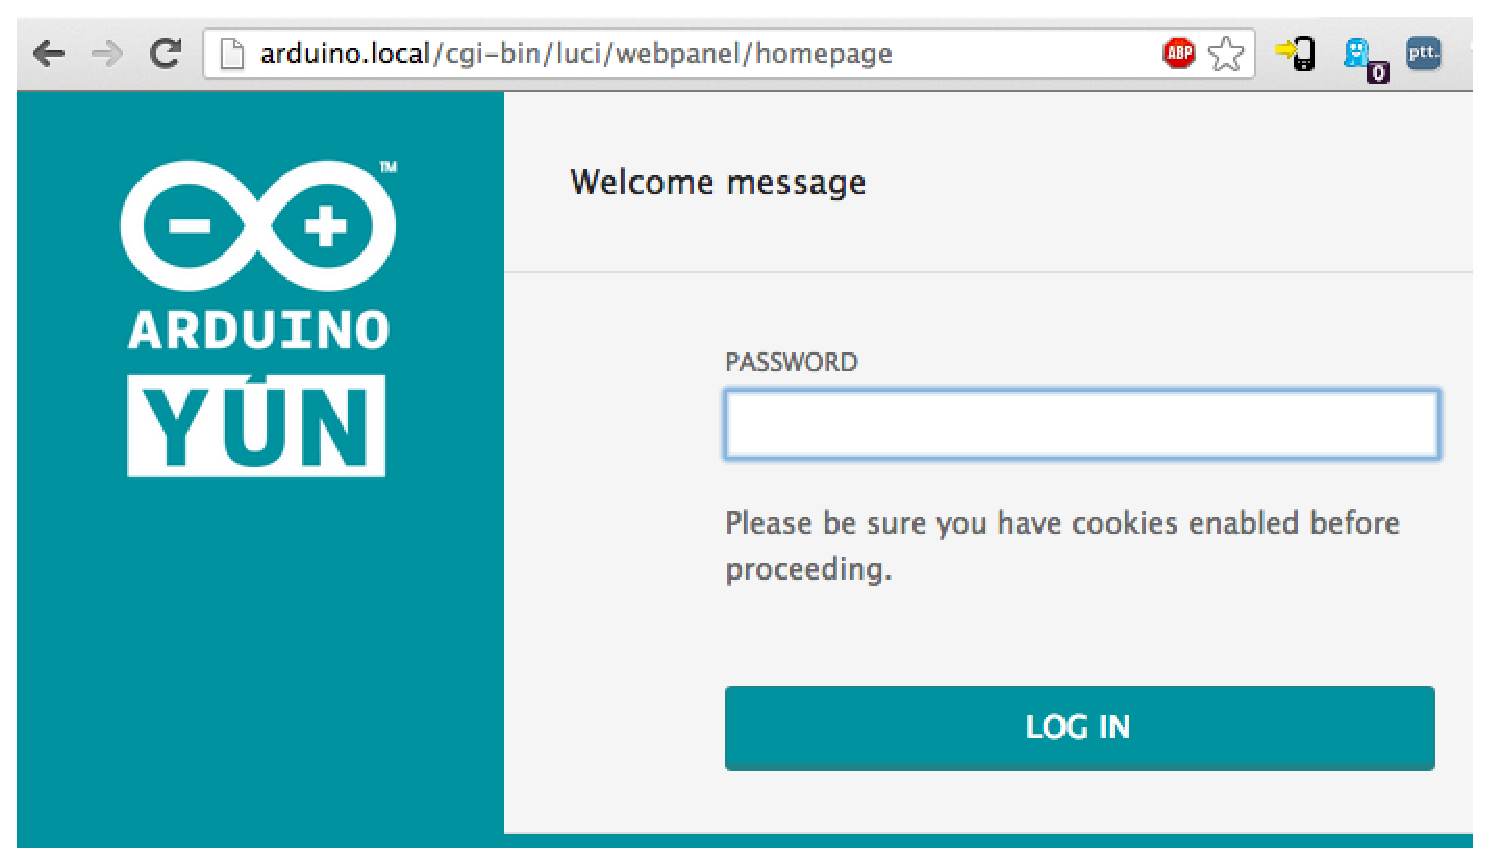
\includegraphics[keepaspectratio,width=0.6\textwidth]{YunWebPassword.eps}
    \caption{Arduino Yún Web Password}\label{fig:yun-web-password}
\end{figure}

La contraseña por defecto es \emph{arduino}; permite acceder al panel de diagnóstico donde se muestra información sobre la red WiFi y la conexión Ethernet. Además, permite acceder al panel de configuración:

\begin{figure}[H]
    \centering
    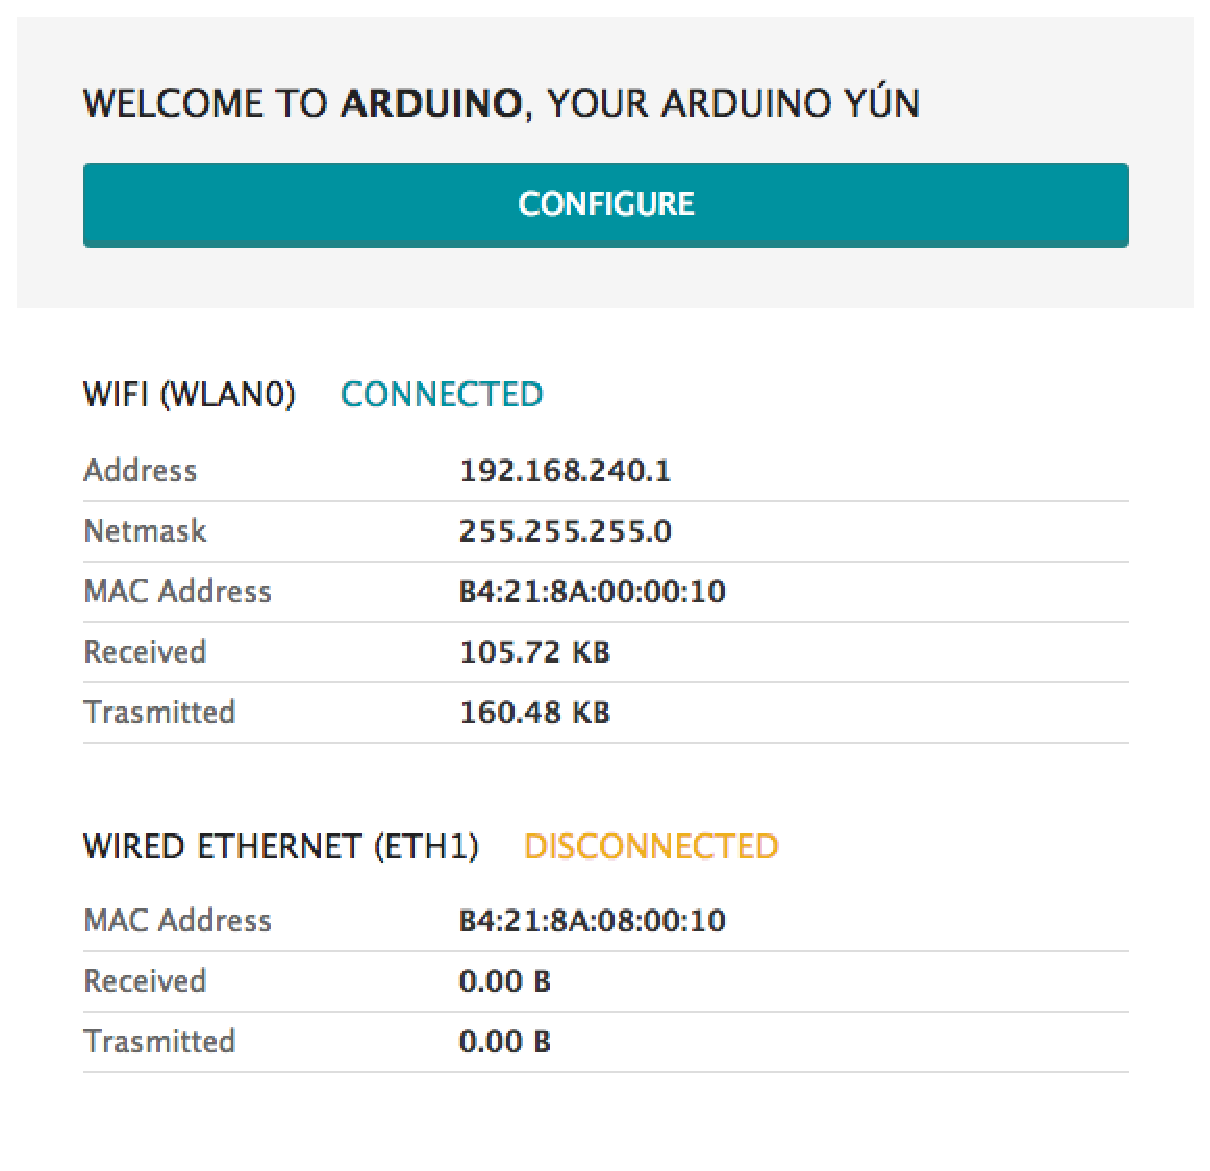
\includegraphics[keepaspectratio,width=0.6\textwidth]{YunWebDiagnostic.eps}
    \caption{Arduino Yún Web Diagnostic}\label{fig:yun-web-diagnostic}
\end{figure}

El panel de configuración permite nombrar nuestra placa Arduino, establecer una contraseña de acceso, configurar la zona horaria y por último, y lo más importante, decirle a que red WiFi debe conectarse.

\begin{figure}[H]
    \centering
    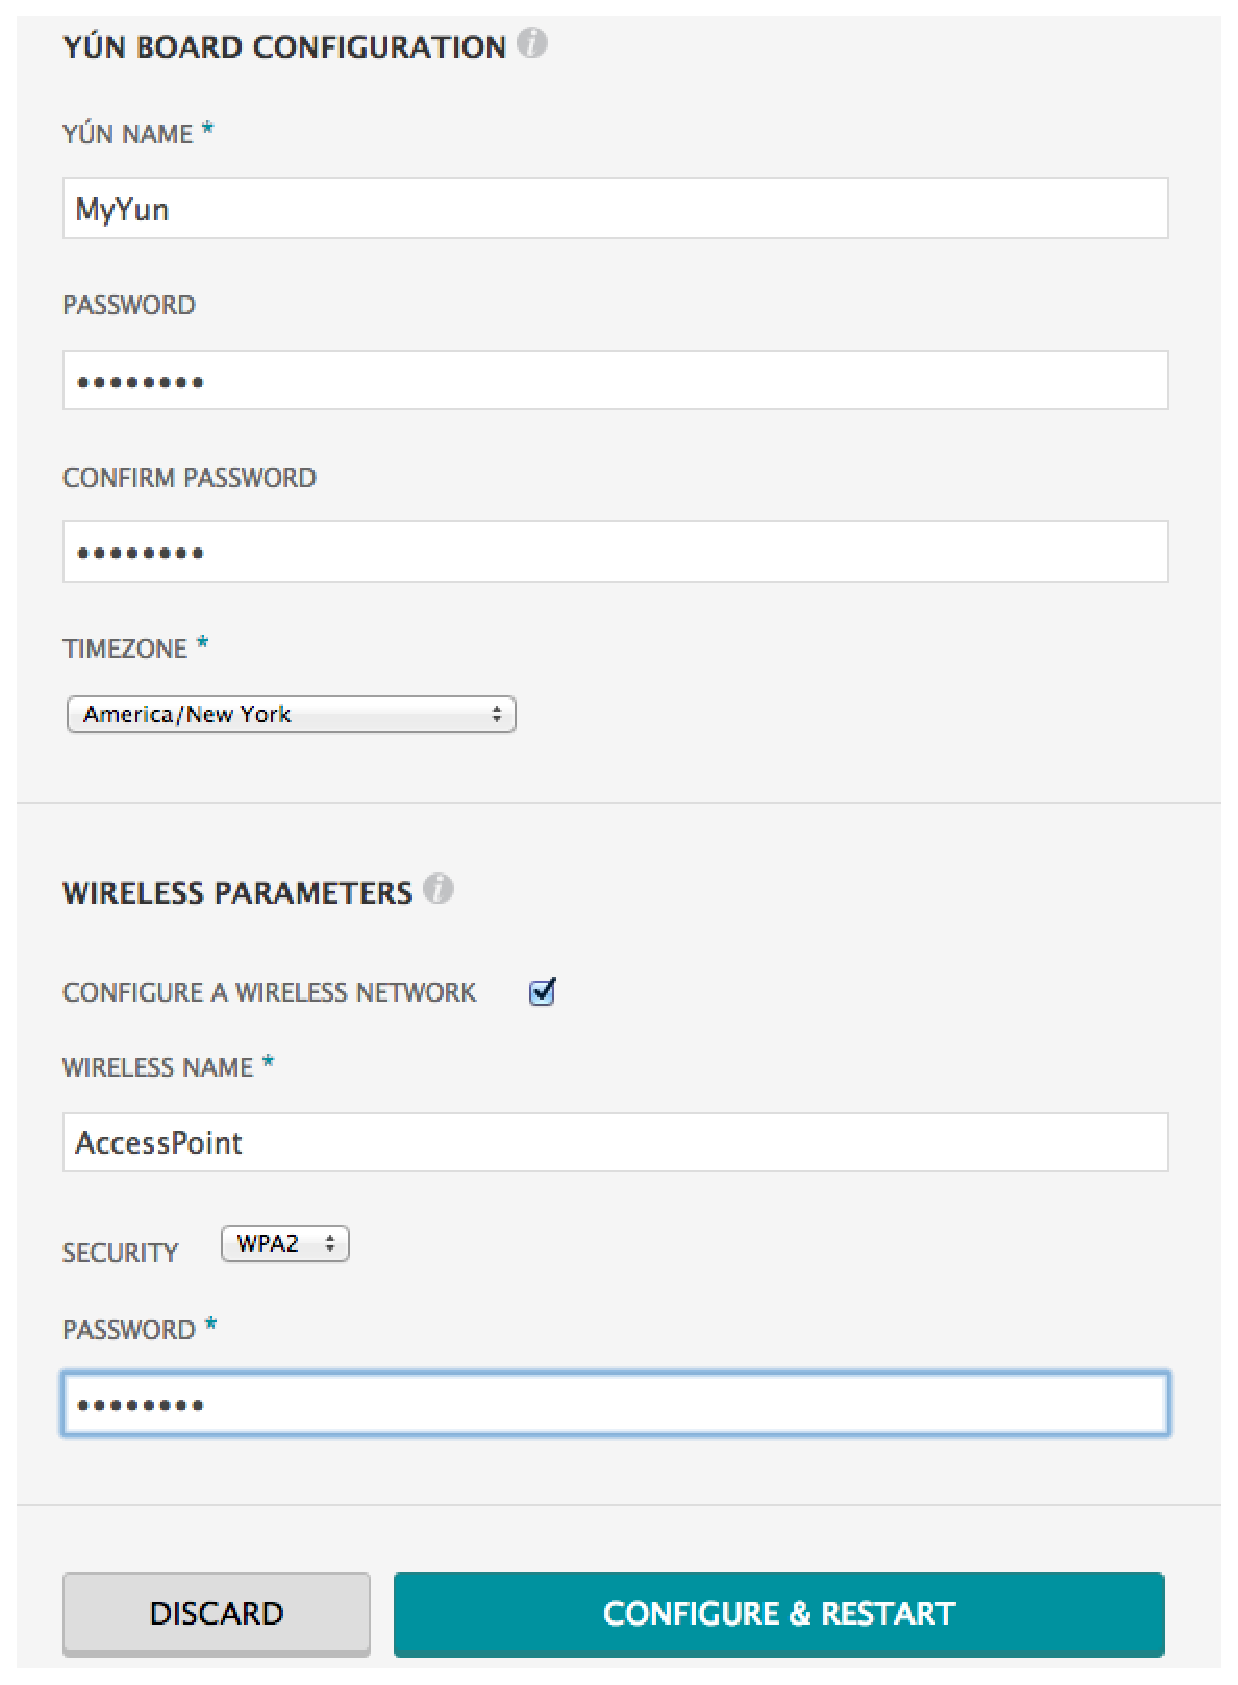
\includegraphics[keepaspectratio,width=0.6\textwidth]{YunWebConfig.eps}
    \caption{Arduino Yún Web Config}\label{fig:yun-web-config}
\end{figure}

Una vez se guarda la nueva configuración la distribución Linux se reinicia y automáticamente se conectará a la red WiFi que hayamos establecido, indicándo a través de un mensaje que se debe volver conectar a la WiFi del usuario:

\begin{figure}[H]
    \centering
    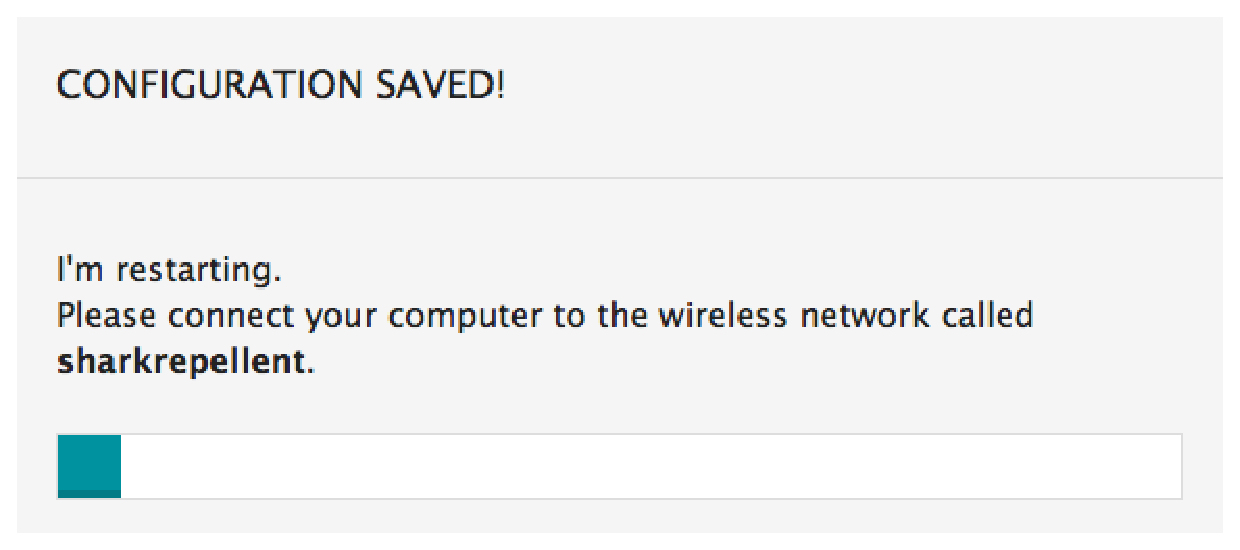
\includegraphics[keepaspectratio,width=0.6\textwidth]{YunRebooting.eps}
    \caption{Arduino Yún Web Rebooting}\label{fig:yun-web-rebooting}
\end{figure}

Pasado varios segundos automáticamente se nos volverá a conectar a la página de configuración de Arduino donde se tendrá que introducir la nueva contraseña para acceder.

\subsection{Problemas detectados}

La versión de Linux que trae la placa Arduino no viene con las librerías para utilizar el puerto USB en modo HID (\emph{Human Interface Device}) por lo que no reconoce el lector de códigos de barras USB. Para configurarlo se han tenido que bajar las librerías e instalarlas a través de SSH.

\begin{enumerate}

    \item Descargar y guardar en la memoria micro-sd (\emph{/mnt/sda1/}) las dos siguientes librerías:

        \begin{itemize}
            \item kmod-hid-generic\_3.8.3-1\_ar71xx.ipk
            \item kmod-hid\_3.8.3-1\_ar71xx.ipk
        \end{itemize}

    \item Actualizar el sistema de paquetes e instalar las dos siguientes librerías para permitir la instalación de las librerías anteriores:

        \begin{lstlisting}
opkg update
opkg install kmod-input-core
opkg install kmod-input-evdev
        \end{lstlisting}

    \item Instalar las librerías de la micro-sd:

        \begin{lstlisting}
rm /tmp/opkg-lists/*
opkg install /mnt/sda1/kmod-hid\_3.8.3-1\_ar71xx.ipk
opkg install /mnt/sda1/kmod-hid-generic\_3.8.3-1\_ar71xx.ipk
        \end{lstlisting}

    \item Instalar el driver HID:

        \begin{lstlisting}
opkg update
opkg install kmod-usb-hid
        \end{lstlisting}

    \item Cargar el driver HID en el Kernel:

        \begin{lstlisting}
insmod hid-generic
echo "hid-generic" >>/etc/modules.d/62-hid-generic
        \end{lstlisting}

    \item Reiniciar Linux:

        \begin{lstlisting}
reboot
        \end{lstlisting}

    \item Enchufar el lector de tarjetas USB y comprobar que funciona:

        \begin{lstlisting}
cat /dev/input/event1 | hexdump
        \end{lstlisting}

\end{enumerate}

Con esta configuración Linux es capaz de cargar el dispositivo USB, pero, si se desenchufa y se vuelve a enchufar a veces no carga y da problemas. Por suerte, el \emph{23 de Abril de 2014} han sacado una nueva versión de \emph{OpenWrt-Yun} que corrige estos errores, e introduce las siguientes mejoras:

    \begin{itemize}
        \item OpenWrt
            \begin{itemize}
                \item wget now supports ssl
                \item Fixed fuses values in run-avrdude
                \item nano is now built-in (no need to become ''vi'' experts any more)
                \item Updated ruby to 1.9.3-p429
                \item Fixed USB port stability (when using it both with a pen drive or as a serial device)
                \item Patched dhcp script to fix ethernet routing issue
                \item Added lots of webcam modules
                \item Fixed USB keyboard support
                \item Heartbleed http://heartbleed.com/
                \item Linux side ready visual notification: when linux boot completes, the usb led lights up (it's bright white)
                \item Disk space expander tutorial: using an micro SD card to have gigabytes of disk space
                \item Added ''upgrade-all'' script for easier massive upgrade of packages (available only after having followed the ExpandingYunDiskSpace tutorial)
                \item Node.js is now available as an optional package: other native nodejs packages include bleno, noble, serialport, socket.io.
            \end{itemize}

        \item Web panel
            \begin{itemize}
                \item Previously, jsonp calls were triggered by the ''jsonp'' query string parameter only. Now, you can use ''callback'' as well.
                \item Added Mailbox support
                \item Various fixes
            \end{itemize}

        \item Bridge
            \begin{itemize}
                \item File.size() now implemented
                \item PHP bridge client (thx Luca Saltoggio)
                \item Bridge is now run with ''-u'' python flag, preventing some random lockups in the Bridge
                \item Resolved conflict with python ''json'' module
            \end{itemize}
    \end{itemize}

Una vez actualizado la versión de \emph{OpenWrt-Yun} siguiendo las instrucciones de la página de Arduino (\emph{http://arduino.cc/en/Tutorial/YunSysupgrade}) solamente se tiene que instalar la librería USB HID por SSH (ya que sigue sin venir por defecto):

    \begin{lstlisting}
opkg update
opkg install kmod-usb-hid
    \end{lstlisting}

Y automáticamente detectará el lector de códigos de barras USB sin ningún problema, aunque se desenchufe y se vuelva a enchufar.

\subsection{Decodificando el lector de código de barras}

El siguiente problema a resolver es la creación de un script en \emph{python} que permita la lectura de códigos de barras. Para ello se ha tenido que decodificar los caracteres que envía al sistema operativo, y una vez hecho, comprender como funciona.

El funcionamiento es muy sencillo. Cuando el lector de código de barras encuentra un código válido lo envía al sistema por letras y por último, y es lo que nos ayuda a comprender que ha terminado de enviarnos el código de barras, nos envía dos caracteres seguidos (\emph{Control + j}) que simbolizan el salto de línea (\emph{Line Feed}).

El siguiente script nos permite leer los caracteres escaneados e imprimirlos por consola o enviarlos al microcontrolador a través de la librería \emph{Bridge}.

\begin{lstlisting}
#!/usr/bin/python
# -*- coding: utf-8 -*-

import struct
import time
import sys
sys.path.insert(0, '/usr/lib/python2.7/bridge/')

from bridgeclient import BridgeClient as bridgeclient

# Variables
infile_path = "/dev/input/event1"

#long int, long int, unsigned short, unsigned short, unsigned int
FORMAT = 'llHHI'
EVENT_SIZE = struct.calcsize(FORMAT)

teclasPulsadas = dict()
escribiendoLetras = False
codigoBarras = ''
bridgeCliente = bridgeclient()
in_file = None

# Funciones

def esTeclaNumerica(value):
    return value >= 458782 and value <= 458791

def getNumero(value):
    return (value - 458781)%10

def esTeclaLetra(value):
    return (value >= 458756 and value <= 458781)

def getLetra(value):
    posicionValue = value - 458756
    asciiValue = posicionValue + 65
    return str(unichr(asciiValue))

# 458792 -> Intro
# 458976 + 458765 (Control + j => Line Feed)
def esTeclaControl(value):
    return value == 458792 or \
            value == 458976 or \
            value == 458765
def procesarEvento(event):
    global teclasPulsadas, escribiendoLetras, codigoBarras, bridgeCliente
    (tv_sec, tv_usec, type, code, value) = struct.unpack(FORMAT, event)

    # Importa este orden de la condicion, si se altera puede imprimir
    # caracteres escritos muy deprisa en otro orden
    if value not in teclasPulsadas:
        teclasPulsadas[value] = 'S'
    else:
        if esTeclaControl(value) and escribiendoLetras:
            escribiendoLetras = False
            print codigoBarras
            #bridgeCliente.put('codebar', codigoBarras)

            codigoBarras = ''
        elif not esTeclaControl(value) and \
                (esTeclaNumerica(value) or \
                esTeclaLetra(value)):
            escribiendoLetras = True
            if esTeclaNumerica(value):
                codigoBarras += str(getNumero(value))
            elif esTeclaLetra(value):
                codigoBarras += getTeclaLetra(value)
        del teclasPulsadas[value]

def conectarUsb():
    global in_file
    in_file = None
    conectado = False
    while not conectado:
        try:
            # Intentamos abrir el fichero
            in_file = open(infile_path, "rb")
            conectado = True
        except IOError:
            time.sleep(1) # Pausamos 1seg

# Inicio programa
conectarUsb()
event = in_file.read(EVENT_SIZE)
while event:
    try:
        procesarEvento(event)
        event = in_file.read(EVENT_SIZE)
    except IOError:
        conectarUsb()
        event = in_file.read(EVENT_SIZE)
\end{lstlisting}

\subsection{Vinculación del lector}

Tras conectar el lector a nuestra red WiFi como se explica anteriormente, lo que se muestra en la pantalla de nuestro lector \emph{Arduino} es un mensaje indicando que se necesita vincular el dispositivo.

\begin{figure}[h!]
    \centering
    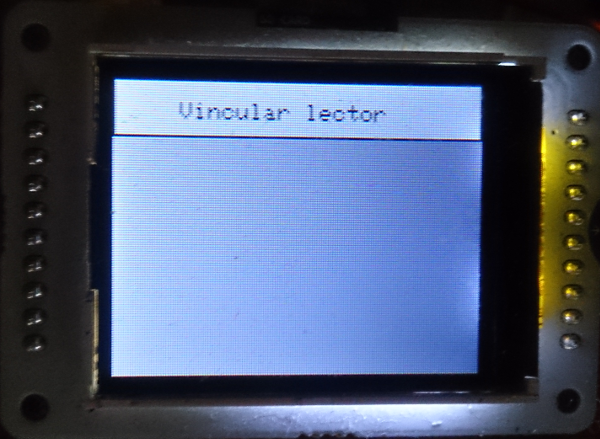
\includegraphics[keepaspectratio,width=0.6\textwidth]{lector_vincular_lector.png}
    \caption{Vincular lector}\label{fig:lector_vincular_lector_1}
\end{figure}


A través de la aplicación web se debe añadir un lector y generar los dos códigos de barras, los cuales se imprimirán para que puedan ser leídos por el lector de código de barras.

Se escanearán con el lector en el orden que se indica en la aplicación web, una vez se han escaneado el lector lanzará una petición para vincularse con nuestra cuenta de usuario. Si el servidor response correctamente, se guarda en la memoria \emph{MicroSD} la clave de acceso pública y se muestra la Home del dispositivo con las opciones disponibles.

En caso de producirse un error se muestra un mensaje para que lo vuelva a intentar.

\subsection{Opciones del lector}

Una vez se ha vinculado el lector, utilizando la clave pública de acceso se lanza una petición para obtener la información del cliente. Con esta información, nombre y frigorificos que dispone, se dibuja la pantalla de inicio con el nombre del cliente, el frigorífico activo seleccionado y las opciones de menú.

    [FOTOGRAFIA PANTALLA INICIO]

El dispositivo cuenta con cuatro botones para manejar el menú colocados en disposición de cruceta y dos botones para \emph{Aceptar} ó \emph{Cancelar} una opción.

A través de los botones podremos navegar por las distintas opciones del lector:

\begin{itemize}

    \item Selección del frigorífico activo

        Esta opción de menú nos permitirá elegir el frigorífico sobre el que se realizarán las acciones (entrada / salida) de productos.

        [FOTOGRAFIA OPCIÓN DE MENÚ]

    \item Modo entrada de productos

        Para introducir productos al frigorífico nos colocaremos en esta opción de menú el cual activará la lectura de productos por \emph{código de barras} ó a través del \emph{lector RFID}.

        [FOTOGRAFIA OPCIÓN DE MENÚ]

    \item Entrada de un producto de forma manual

        Debido a las limitaciones del lector de código de barras hay algunos productos que presentan dificultades para ser escaneados, en concreto, aquellos cuyos códigos de barras sean muy pequeños o estén localizados en zonas curvas.

        Por ello, se permite la introducción manual del código de barras utilizando para ello la cruceta:

        [FOTOGRAFIA OPCIÓN DE MENÚ]

    \item Modo salida de productos

        Para sacar productos del frigorífico nos colocaremos en esta opción del menú el cual activará la lectura de productos por \emph{código de barras} ó a través del \emph{lector RFID}.

        [FOTOGRAFIA OPCIÓN DE MENÚ]

    \item Salida de un producto de forma manual

        Al igual que a la entrada de productos se pueden presentar problemas para escanear un producto, sucede lo mismo a la salida del producto, por lo que se da la misma opción para introducir el código de barras de manera manual.

        [FOTOGRAFIA OPCIÓN DE MENÚ]

    \item Desvinculación del aparato

        Esta opción de menú borrará de la memoria \emph{MicroSD} la clave pública de acceso, con lo cual se quedará desvinculado el lector de nuestra cuenta de usuario en la aplicación web.

        Para volver a utilizar el lector será necesario volver a enlazarlo.

        [FOTOGRAFIA OPCIÓN DE MENÚ]

\end{itemize}